% !TeX root = ../FinalRepordCS.tex

\chapter{Implementation and Preliminary Performance Analysis}

\section{Implementation}
In this section, the primary emphasis is on executing the functionalities of LoRa nodes Alice and Bob by leveraging the Arduino programmable MCU board and IDE previously discussed. This implementation is conducted in tandem with the LoRa frequency modulation chip and the algorithms outlined earlier.

\begin{figure}
  \centering
  \subcaptionbox{LoRa Node Implementation\label{LoraNodeImplate}}
  {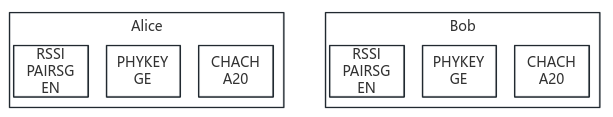
\includegraphics[width=0.8\linewidth]{LoraImplate.png}}
  \subcaptionbox{LoRa Transmission Implementation\label{LoraTransimissionImplate}}
  {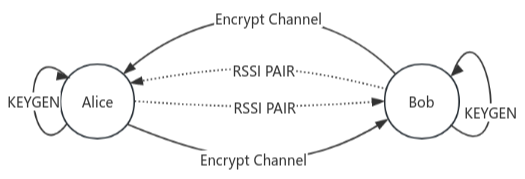
\includegraphics[width=0.7\linewidth]{LORAtransmit.png}}
  \caption{Implementation Details}\label{Implementation Details}
\end{figure}

As depicted in Figure \ref{Implementation Details}, the LoRa nodes primarily executed the following functions:

\begin{itemize}
  \item Generation of RSSI key pairs 
  \item Generation of physical layer bit codes
  \item Implementation of Chacha20 encryption and decryption
\end{itemize}

Additionally, the transmission protocol for the physical layer key and encrypted communication channel has been realized, encompassing:

\begin{itemize}
  \item A half-duplex-based protocol for exchanging RSSI pairs  
  \item Chacha20-based transmission for the LoRa Protocol
\end{itemize}


\section{Deep-in-Building and Outdoor Test}
Following the implementation of the LoRa nodes, a practical test was conducted to generate LoRa physical layer keys within real-world application scenarios, encompassing both Deep-in-Building and Outdoor Tests. The test produced a wealth of results, providing tangible evidence for the practical applicability of LoRa in real-world settings. These findings hold significant reference value, serving to inform and guide the future deployment of the LoRa protocol, especially in the context of environmental monitoring.

As shown in Figure \ref{conghuatest}, in Liangkou Town, Conghua District, Guangzhou City, there is a sampling point (Bob) deployed on a communication tower for monitoring high-precision greenhouse gas flux. It is situated at an approximate height of 50 meters. Alice conducted an outdoor test from a temple located at a linear distance of around 300 meters from Bob.
Meanwhile, Figure \ref{panyutest} represents an outdoor test conducted at the central area of Guangzhou Higher Education Mega Center. This test involved a combination of stationary and mobile scenarios.
\begin{figure}
  \centering
  \subcaptionbox{Conghua out door test\label{conghuatest}}
  {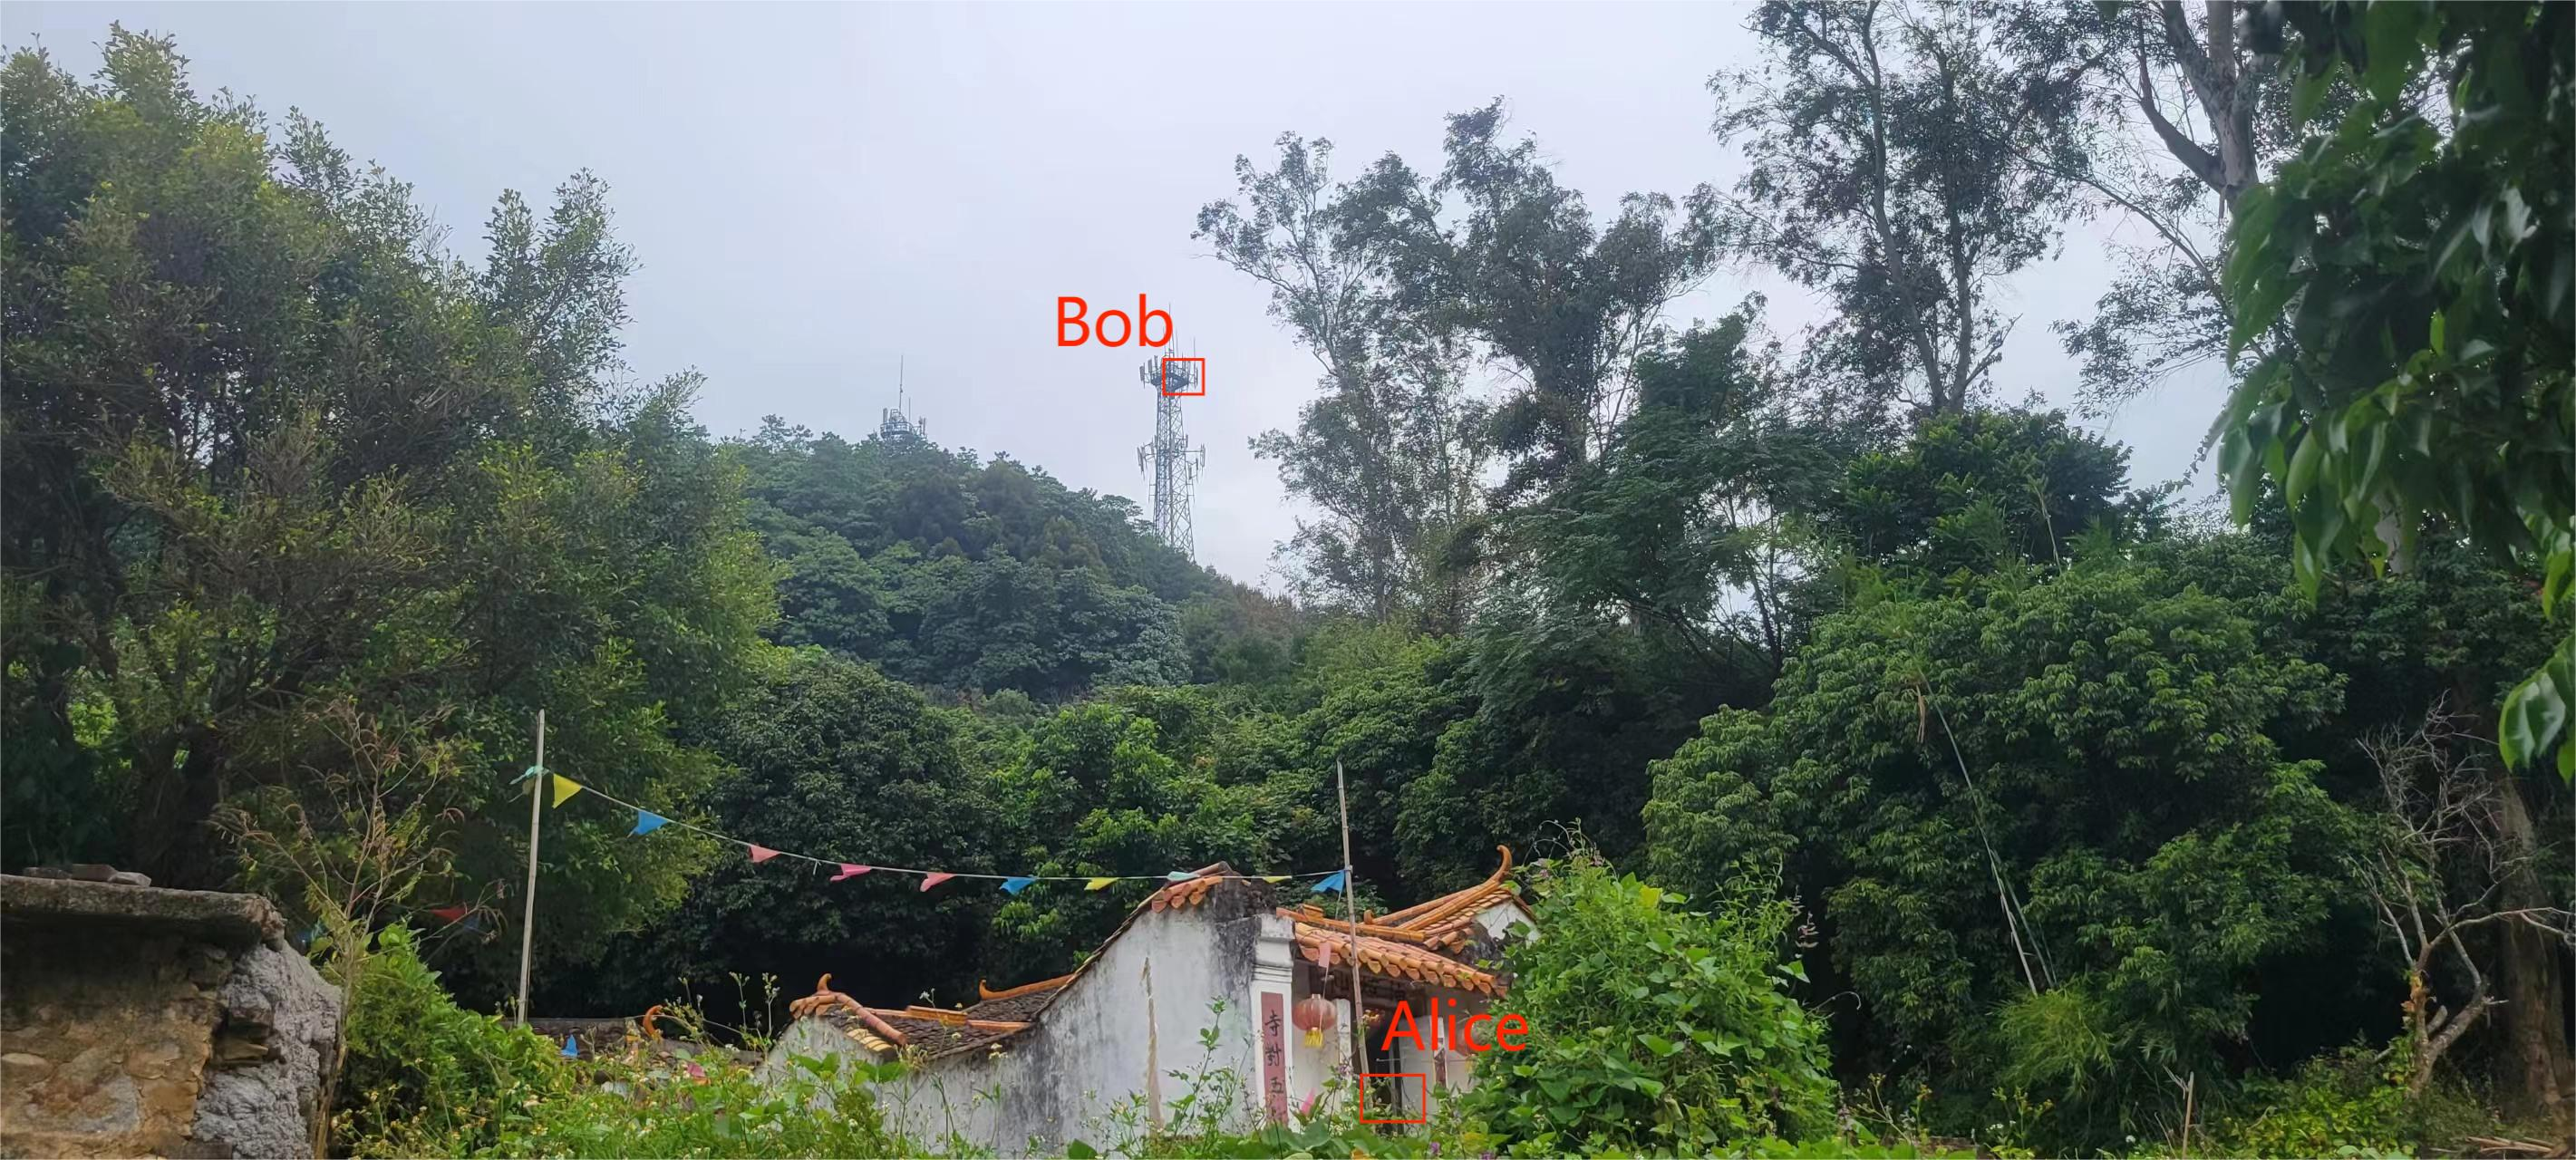
\includegraphics[width=0.8\linewidth]{conghua.jpg}}
  \subcaptionbox{Panyu out door test\label{panyutest}}
  {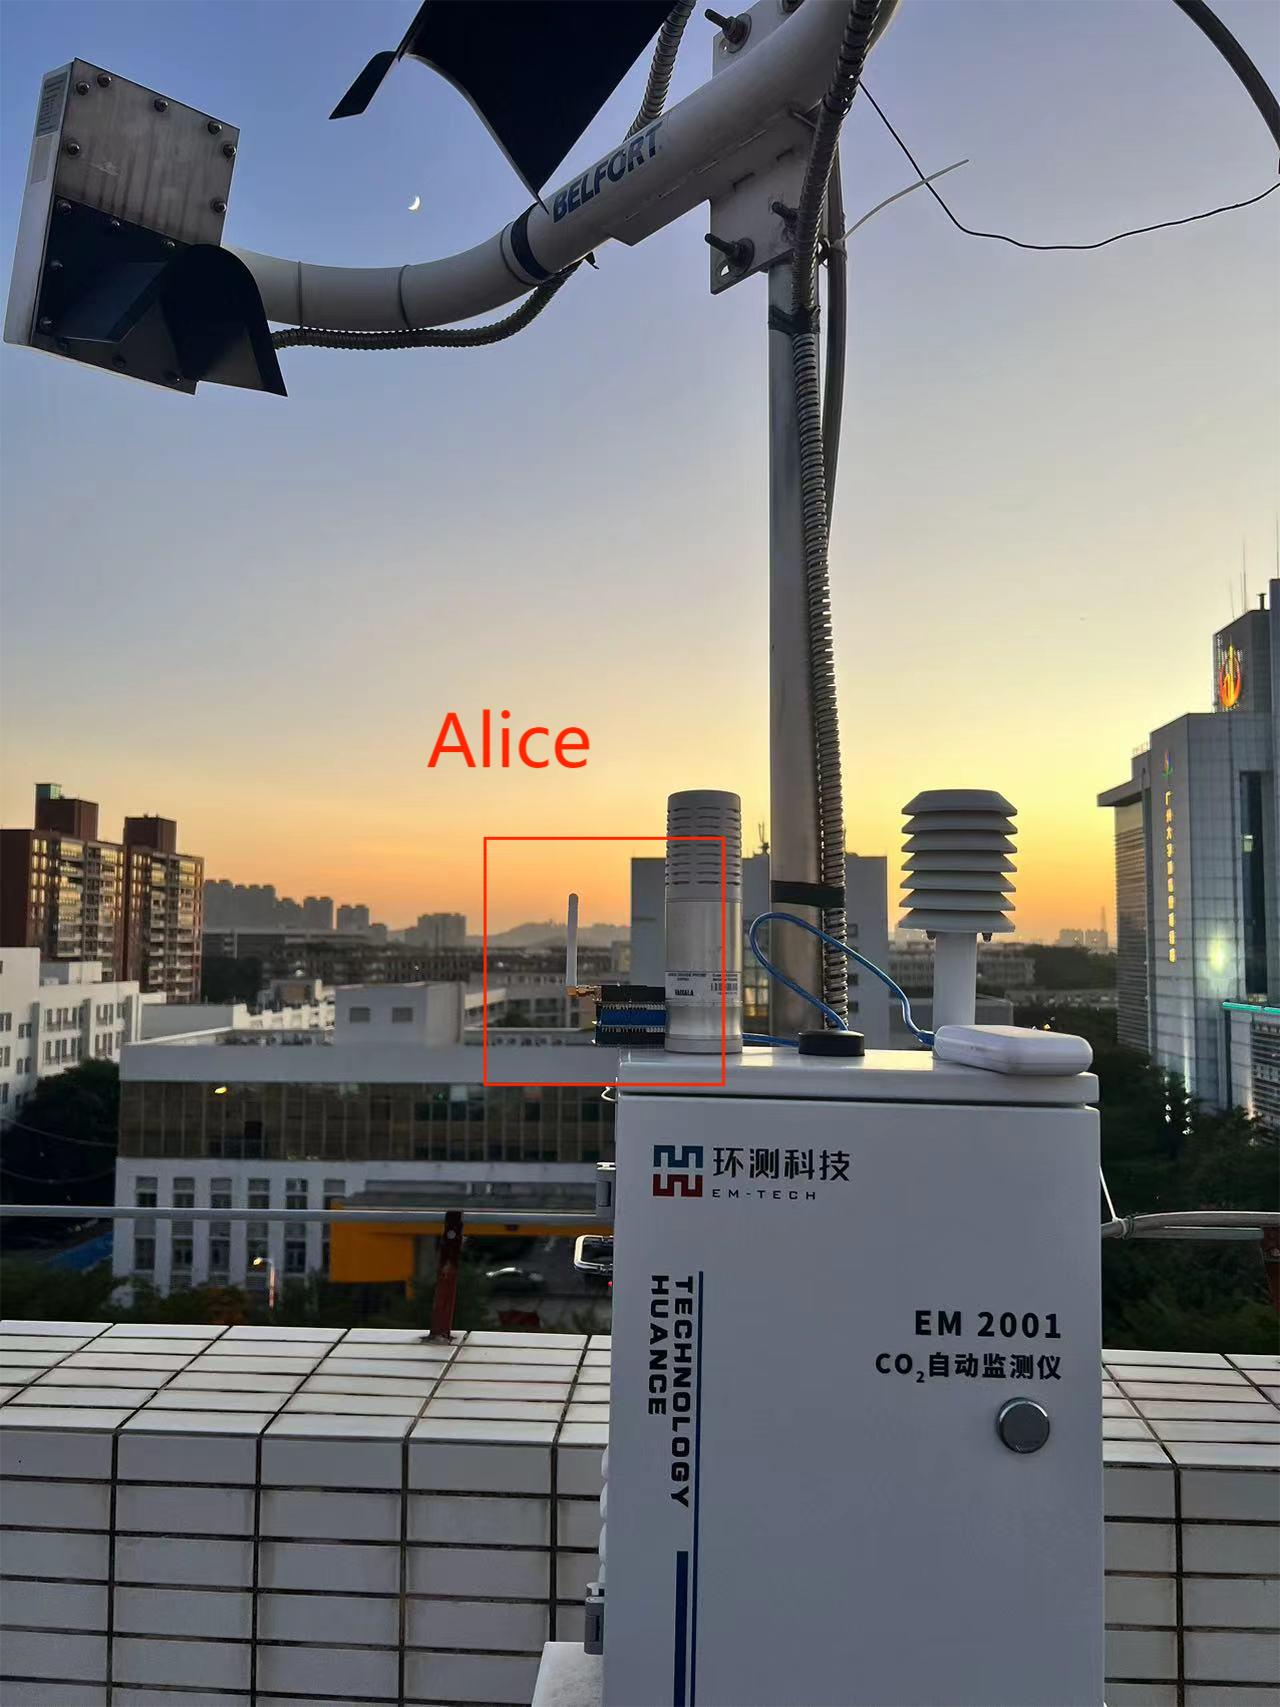
\includegraphics[width=0.3\linewidth]{panyuhighereducationmegacenter.jpg}}
  \subcaptionbox{Near instruments test\label{neartheinstruments}}
  {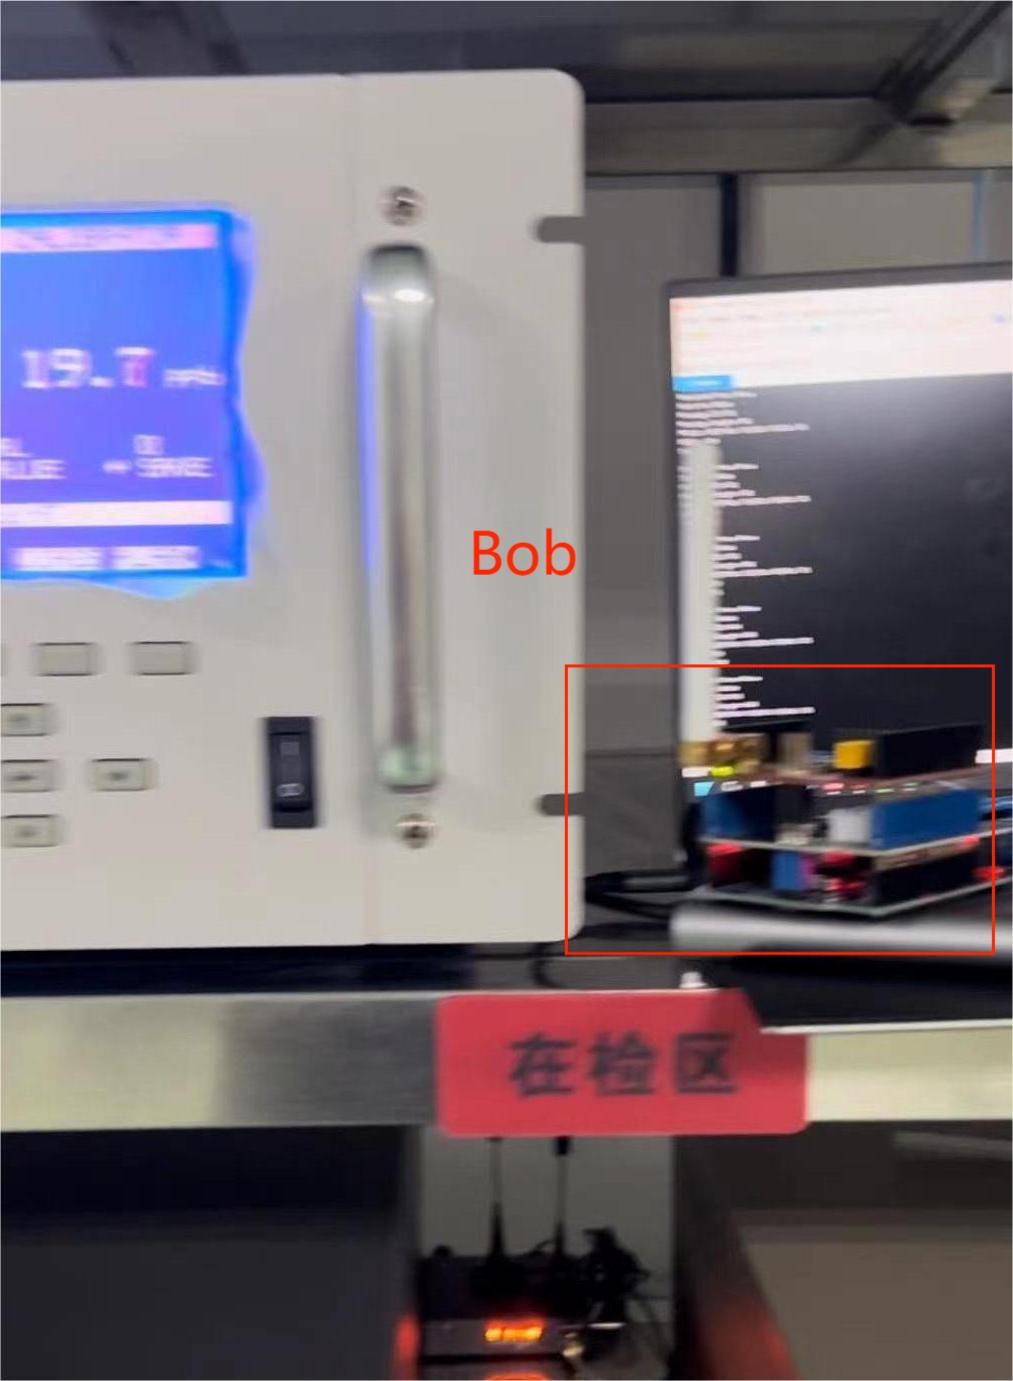
\includegraphics[width=0.3\linewidth]{neartheinstruments.jpg}}
  \subcaptionbox{In building test\label{inbuildingtest}}
  {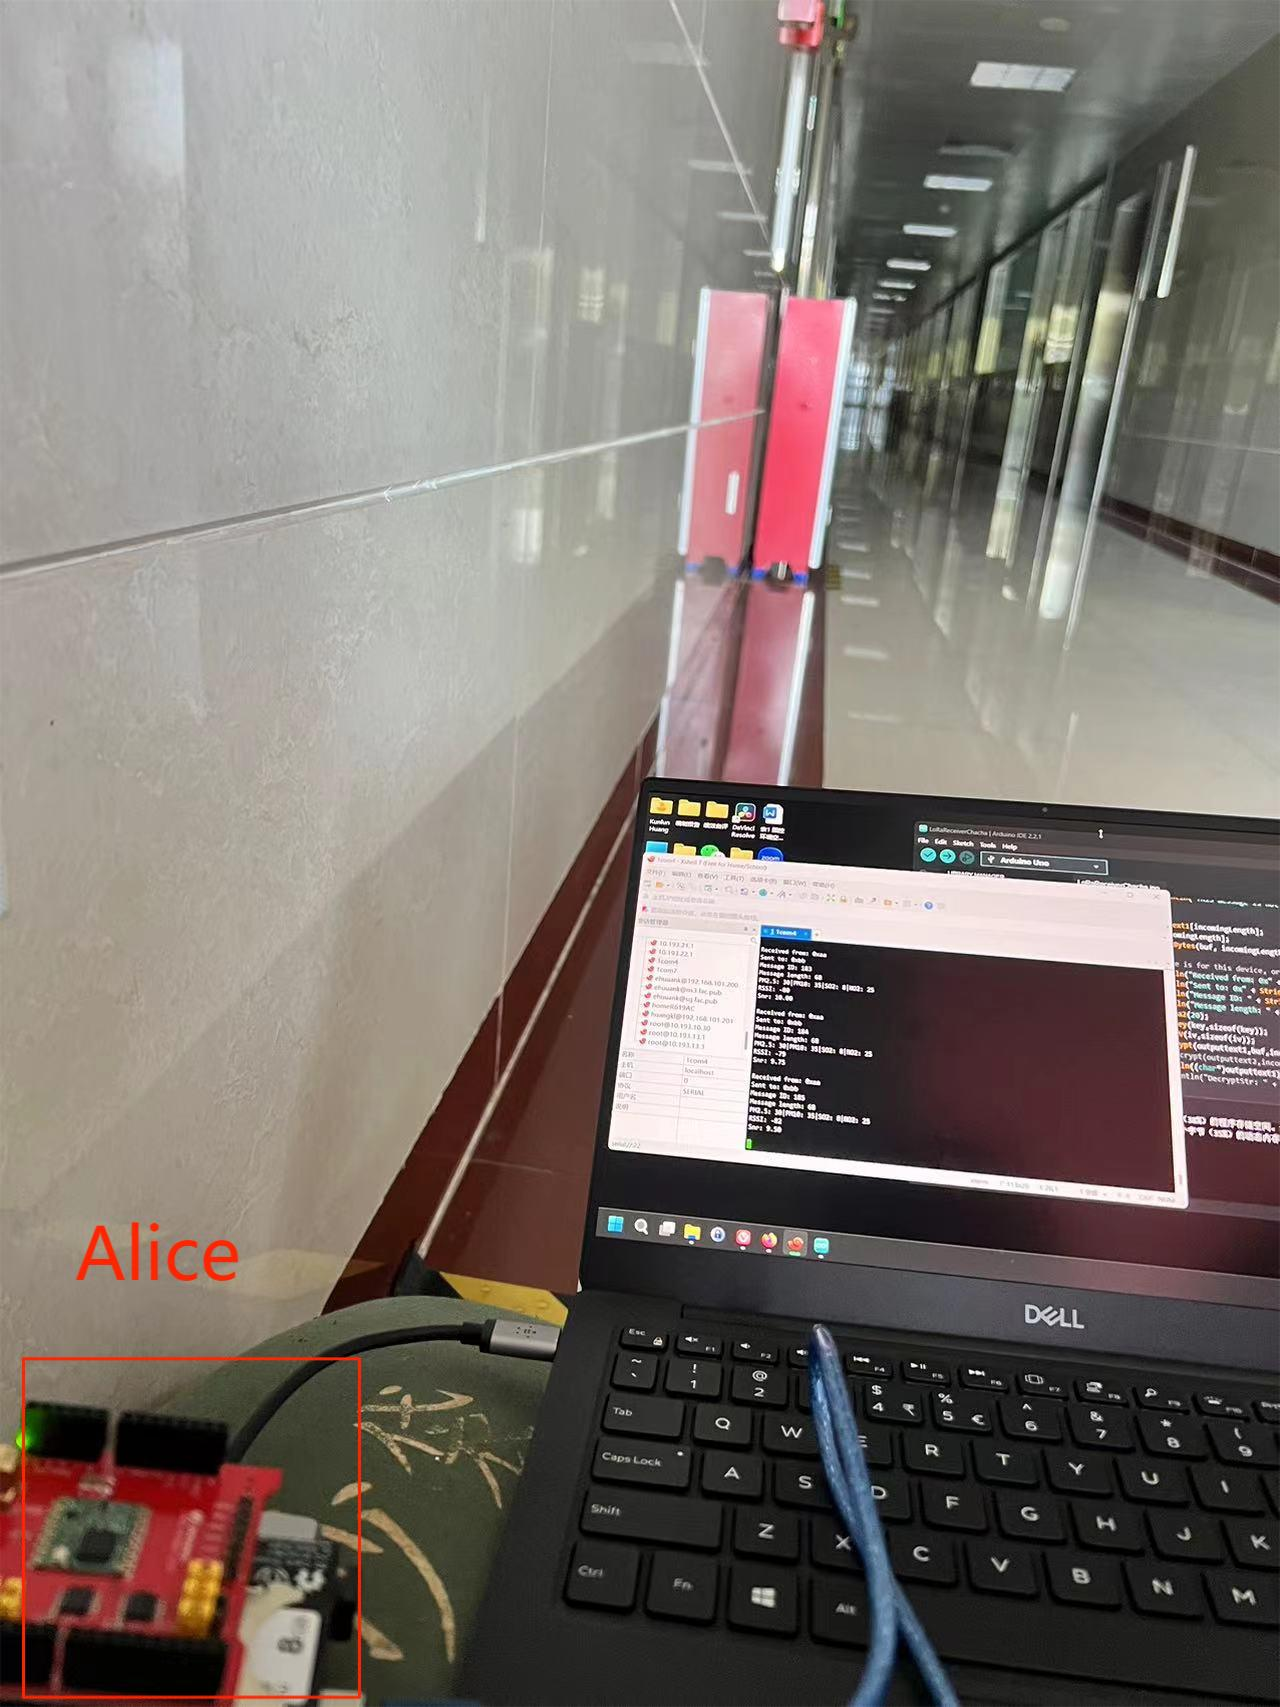
\includegraphics[width=0.3\linewidth]{inbuildingtest.jpg}}
  \caption{Deep-in-Building and Outdoor Test}\label{Test}
\end{figure}

Simultaneously, numerous tests were conducted indoors, especially in situations involving high-power instruments and electromagnetic field interference.
\subsection{RSSI Pairs Generation}
Through the aforementioned tests, our LoRa nodes utilized a half-duplex-based protocol for exchanging RSSI pairs. We collected a significant dataset, obtaining data in the form of \(n\) pairs \(\underbrace{\{RSSI_{Alice}^1, RSSI_{Bob}^1\}...\{RSSI_{Alice}^n, RSSI_{Bob}^n\}}_{n\_pairs}\) through the serial port or Arduino's storage card. Figure \ref{sampling5} shows the serial port displaying the sampling in LoRa Node.
\begin{figure}
  \centering
  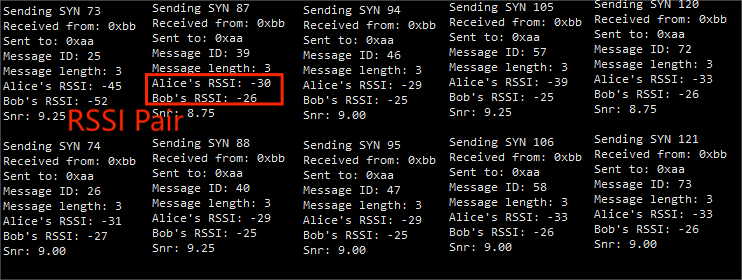
\includegraphics[width=0.9\linewidth]{sampling5.png}
  \caption{Sampling in LoRa Node}
  \label{sampling5}
\end{figure}

However, due to the influence of various factors such as physical constraints, environmental conditions, communication distances, etc., further processing is required for the generated RSSI pairs.

\subsection{Key Generation}
Than a program that implemented constitutes a crucial section of the thesis, focusing on LoRa physical layer key generation. Beginning with the processing of RSSI data for both Alice and Bob, the code subsequently employs linear interpolation and Savitzky-Golay filtering to enhance the quality of the data.

Following these preprocessing steps, the script employs $M-ary$ quantization on the smoothed RSSI values, utilizing a specified number of bits per sample and an alpha parameter. The homotopy method for error correction is then implemented, where a matrix \(A\) and vector \(y\) undergo iterative updates to correct errors in the data.

The key generation process involves the random generation of a matrix \(A\), the computation of vectors \(y_1\) and \(y_2\) based on the quantized data from Alice and Bob, and the application of error correction through the homotopy method. The final step involves XORing the original bits with the corrected bits to derive the cryptographic key.

The code also incorporates visualizations using Matplotlib to illustrate the impact of linear interpolation and Savitzky-Golay filtering on the original RSSI values. Additionally, the thesis section concludes with the presentation of crucial output information, including filtered RSSI arrays for Alice and Bob, and the original and corrected keys for Alice.
\begin{figure}
  \centering
  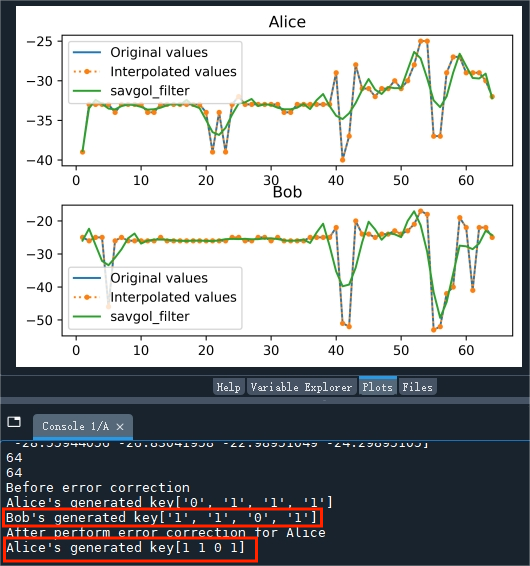
\includegraphics[width=0.8\linewidth]{physicalkeygen.png}
  \caption{Result of Performing Key Generation}
  \label{physicalkeygen}
\end{figure}

Figure \ref{physicalkeygen} illustrated the Key generation results with the multilevel quantization and error correction.

\subsection{Data Encrypt and Decrypt}
Once the key has been generated, it can be employed alongside encryption algorithms to secure the data for transmission.

\begin{figure}
  \centering
  \subcaptionbox{Alice\label{Alice}}
  {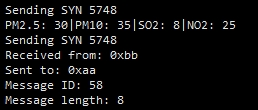
\includegraphics[width=0.4\linewidth]{chachaalice.png}}
  \subcaptionbox{Bob\label{Bob}}
  {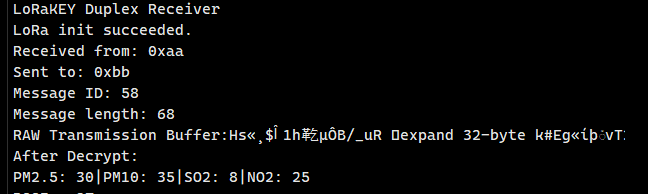
\includegraphics[width=0.7\linewidth]{chachabob.png}}
  \caption{Data Encrypt and Decrypt between Alice and Bob}\label{Data Encrypt and Decrypt}
\end{figure}

\section{Performance Analysis}
In this section, performance tests on password generation were implemented based on references, exploring the impact of different parameters. Additionally, the results were visualized for better comprehension of the test data.
